\section{Meshes}

Test cases run on the following meshes:
\begin{description}
\item[No orography]
\item[Basic terrain following (BTF)]
\item[Smooth level vertical (SLEVE)]{From Sch{\"a}r et al 2002 -- not looked at this for gravity waves test (yet)}
\item[snapCol]{add2dMountain used to snap points underground to the surface, then use snappyHexMesh to remove cells underground by intersecting with surface patch}
\item[snap]{snappyHexMesh applied to unmodified blockMesh.  I also tried making this slightly more orthogonal by modifying the blockMesh with add2dMountain.  Points nearest the surface were moved vertically to meet the surface.  See comparison in Figure~\ref{fig:snap-mesh-compare}.  I haven't run any tests against this mesh (yet) though.}
\end{description}

\begin{figure}
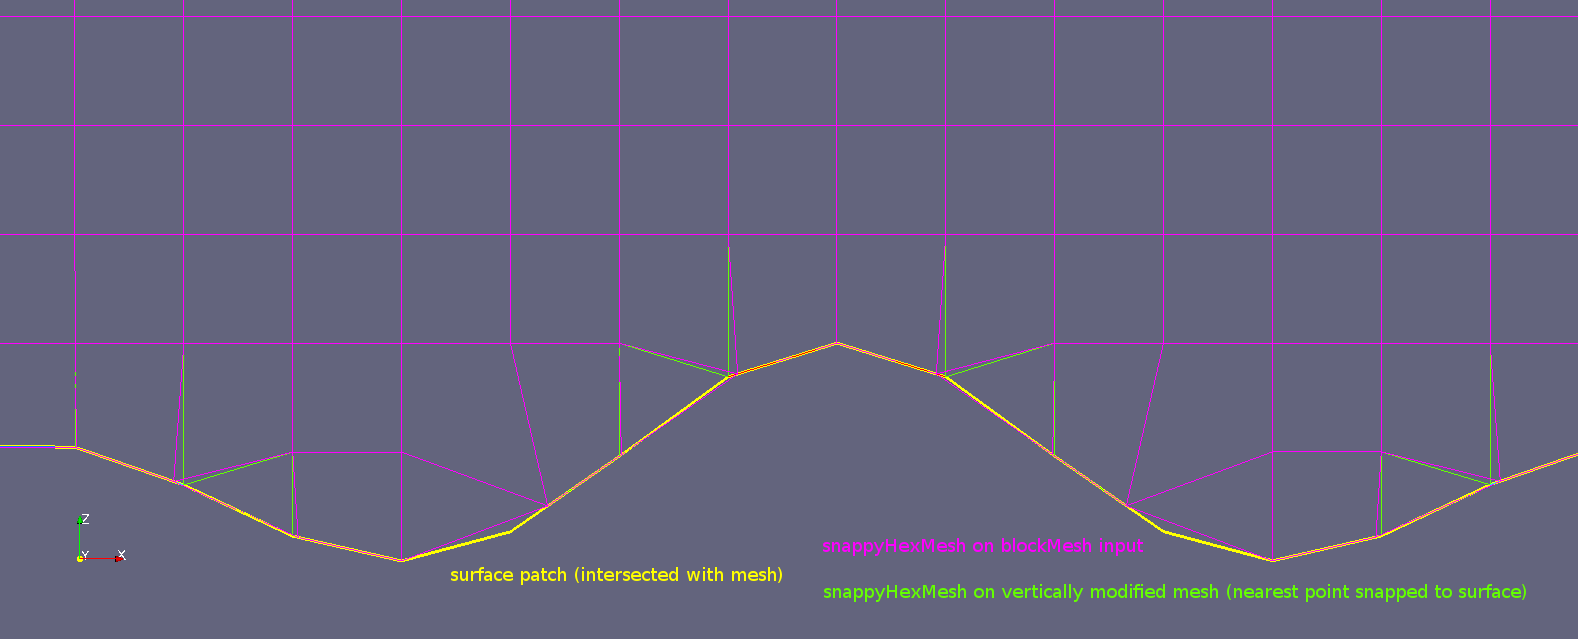
\includegraphics[width=\textwidth]{interim-results/cutCellWarpToSurfaceSchaerExp.png}
\caption{Comparison of snappyHexMesh on blockMesh versus snappyHexMesh after adjustment by add2dMountain.  The latter is more orthogonal.}
\label{fig:snap-mesh-compare}
\end{figure}
